\documentclass{article}

\usepackage[%
    left=0.5in,%
    right=0.5in,%
    top=0.5in,%
    bottom=0.5in,%
]{geometry}%
\usepackage{minitoc}
\usepackage{multicol}
\usepackage{graphicx}
\usepackage{fixltx2e}
\usepackage{listings}
\usepackage{color}
\usepackage{verbatim}
\usepackage{hyperref}
    \hypersetup{ colorlinks = true, linkcolor = blue }
\usepackage{blindtext}
\definecolor{lightgray}{gray}{0.9}
\graphicspath{ {./} }

\newcommand{\inlinecode}[2]{\colorbox{lightgray}{\lstinline
[language=#1]$#2$}}
\newcommand{\worddef}[1]{\hyperref[sec:reference]{\textit{#1}}}

\begin{document}
\section{Spanning tree vs Minumum spanning tree}
\begin{itemize}
	\item Spanning Tree
	\begin{itemize}
		\item Input: connected, undirected graph
		\item Output: a tree which connects all vertices in the graph using only the edges present in the graph
	\end{itemize}
	\item Minimum Spanning Tree
	\begin{itemize}
		\item Input: connected, undirected, weighted graph
		\item Output: a spanning tree
		\begin{itemize}
			\item connects all vertices in the graph using only the edges present in the graph without any cycles and with the minimum possible total edge weight.
			\item is minimum in the sense that the sum of weights of the edges is the smallest possible for any spanning tree
		\end{itemize}
	\end{itemize}
	\item The main difference is that shortest path looks for a lowest cost distance between two nodes, where as \textbf{MST} looks for a shortest path that would go trough all of given vertices 
\end{itemize}
\begin{center}
	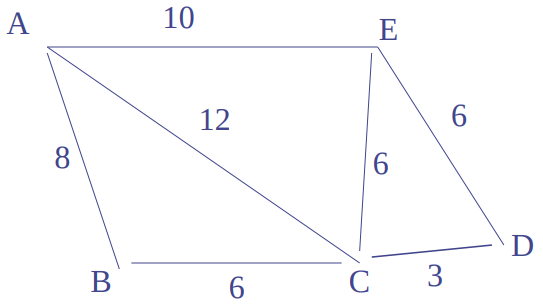
\includegraphics[scale=0.3]{graph.png}
\end{center}
\begin{center}
	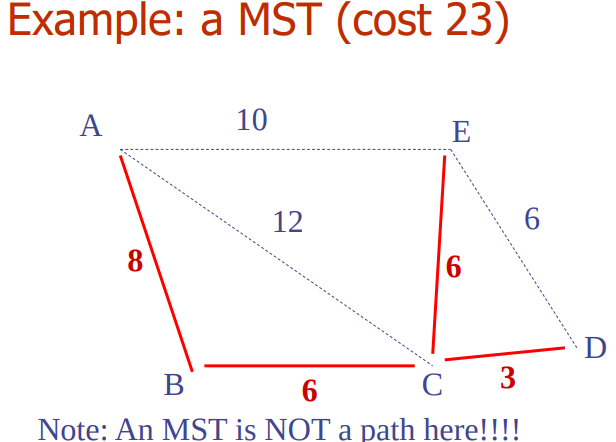
\includegraphics[scale=0.3]{mst.png}
\end{center}
\section{Why MST is a tree}
\begin{flushleft}
We really want a minimum spanning \textbf{sub-graph} ,that is, a subset of the edges that is connected and that contains \textbf{every node}. (Assuming all weights are non-negative) If the graph has a cycle then we can remove an edge of the cycle, and the graph will still be connected, and will have a smaller weight • If a graph is \textbf{connected} and \textbf{acyclic} then it is a tree
\end{flushleft}

\section{Prim's algorithm for constructing MST}
\begin{itemize}
	\item Start by picking any vertex \textbf{M}
	\item hoose the shortest edge from M to any other vertex N
	\item Add edge (M,N) to the MST
	\item Loop:
	\begin{itemize}
		\item Continue to add at every step a shortest edge from a vertex in MST to a vertex outside, until all vertices are in MST
		\item (If there are multiple shortest edges, then can take any arbitrary one)
	\end{itemize}
\end{itemize}

\subsection{Greedy algorithm}
\begin{itemize}
	\item Prim’s algorithm for constructing a Minimal Spanning Tree is a \textbf{greedy algorithm :}
	\item it just adds a minimum weight edge
	\item without worrying about the overall structure, without looking ahead.
	\item It makes a locally optimal choice at each step
\end{itemize}

\section{Proof of MST being optimal}
\begin{comment}
\begin{flushleft}
Assume that exists \textbf{MST} with \texttt{e}. Removing \texttt{e} from it, splits tree in two parts. Expecially, it splits cycle nodes into \textbf{two non empty parts}, call them \texttt{A} and \texttt{B}. Since these nodes form a cycle there is at least one more edge between \texttt{A} and \texttt{B} nodes, call it \texttt{f}. Then MST-e+f is a spanning tree with weight less than MST. That means it is not possible to have MST with e.
\end{flushleft}
\end{comment}

\begin{itemize}
	\item Let \texttt{G} be a weighted connected graph
	\item let \texttt{V1} and \texttt{V2} be a partition of the vertices of \texttt{G} into two \textbf{disjoint non-empty} sets.
	\item Furthermore, let \texttt{e} be an edge with \textbf{minimum weight} from among those with one endpoint in \texttt{V1} and the other in \texttt{V2}.
	\item There is an MST that has e as one of its edges.”
\end{itemize}

\subsection{Justification}
\begin{itemize}
	\item Suppose our MST \texttt{T1} does not include \texttt{e}
	\item We add \texttt{e} to \texttt{T1}, which creates a cycle
	\item That means that tree \texttt{T1} must have some edge  \texttt{e1} that connects \texttt{V1} and \texttt{V2}, 
	\item if we remove \texttt{e1} we now have a tree \texttt{T2} that has lower cost, which means \texttt{T1} was not MST
\end{itemize}

\pagebreak
\section*{Reference section} \label{sec:reference}
\begin{description}
	\item[placeholder] \hfill \\
\end{description}
\end{document}
